\subsection{Solução}

Em resposta à necessidade dos LIMS aumentarem a eficiência de obtenção de dados, foi criada uma solução de workflows dinâmicos, que mudam a forma como as informações são apresentadas e disponibilizadas ao usuário.
Com uma interface adaptável e intuitiva, a solução permite ao usuários acessar e interagir com informações essenciais de maneira rápida e eficiente, melhorando a experiência do usuário.

O usuário tem a possibilidade de escolher, dentre todas as atividades disponíveis para sua visualização, a centralização da atividade escolhida para que ela seja o ponto central do fluxo de trabalho. Com isso, o usuário pode facilmente navegar para outras áreas relevantes da interface e personalizar o fluxo de trabalho de acordo com suas necessidades específicas de forma mais rápida do que seguindo o fluxo de trabalho original.

A rápida disponibilização de informações ao usuário resulta em uma série de ganhos, incluindo maior eficiência dos trabalhos feitos dentro do LIMS, já que workflows podem ser feitos com essa funcionalidade em mente, menor gasto com treinamento no uso do LIMS, já que uma interface dinâmica pode deixar a navegação mais intuitiva e aumento da produtividade do usuário com as informações disponibilizadas mais rapidamente.

O usuário deve, no entanto, saber onde as informações estão contidas dentro do fluxo do trabalho existente para selecionar a atividade correta que contém as informações desejadas. Com isso, a interface se altera para que o fluxo de trabalho seja centralizado na atividade que o usuário deseja.

As informações são disponibilizadas como se a atividade centralizada virasse a atividade inicial do workflow, ocorrendo um ``giro'' da atividade selecionada, transformando a atividades pais em atividades filhas da mesma, como podemos ver na figura~\ref{fig:primeira_implementacao}.

\begin{figure}
    \centering
    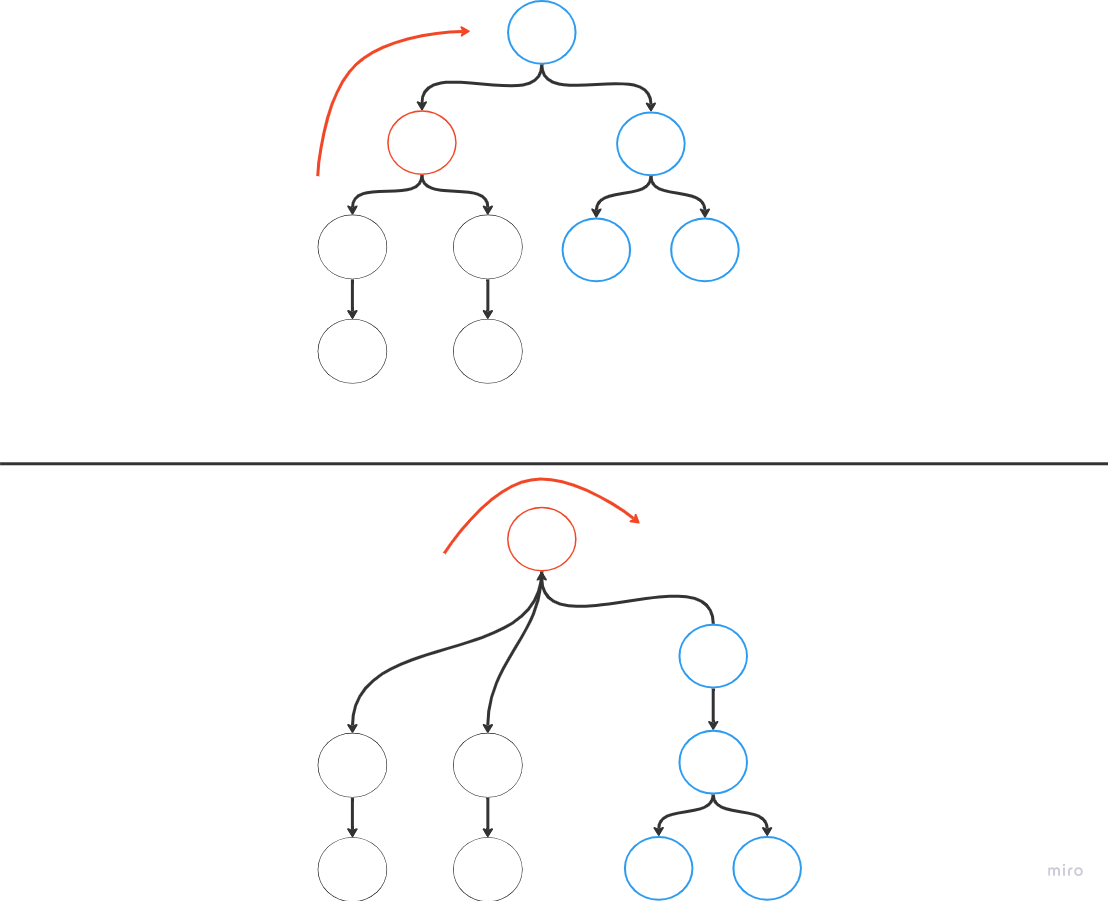
\includegraphics[width=1\textwidth]{imgs/Implementacoes/primeiraImplementacao.png}
    \caption{Representação da implementação de workflows dinâmicas. Na imagem de cima, podemos ver a implementação original de um workflow genérico que está prestes a ser reconstruído. A atividade em vermelho será utilizada como atividade focada apelo usuário. Com isso, a seta em vermelho representa o ``giro'' que o workflow faz para que a atividade selecionada vire a primeira atividade do workflow.}
    \label{fig:primeira_implementacao}
\end{figure}

